\documentclass{standalone}
\usepackage{tikz}
\usetikzlibrary{chains, fit, positioning}

\begin{document}
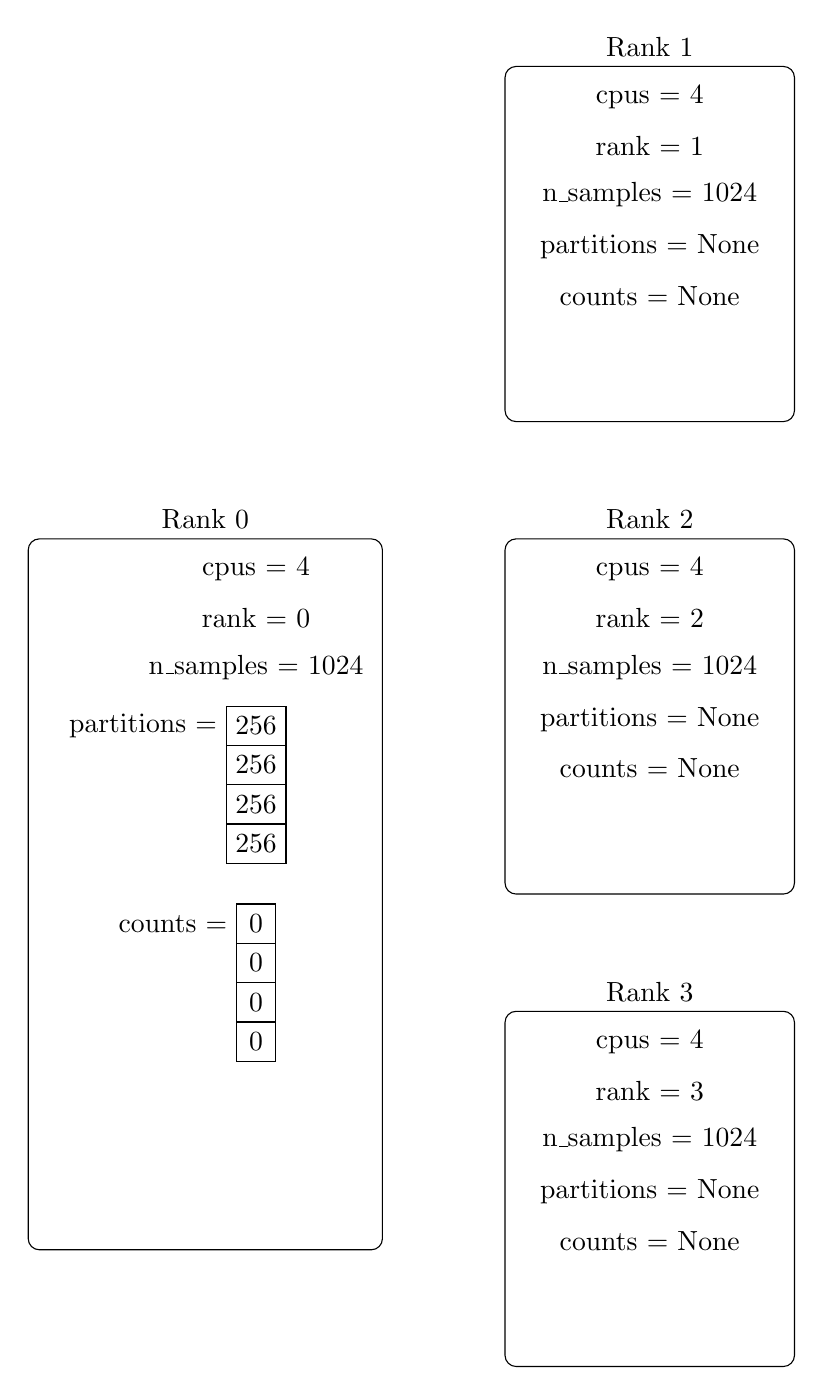
\begin{tikzpicture}
\tikzset{
  arrow/.style={
    >=latex
  },
  line/.style={
    draw,
    ->,
    very thick,
  },
  array/.style={
    draw,
    minimum size=0.5cm
  },
  new/.style={
    red,
    font=\bfseries
  },
  old/.style={
  }
}

% Globals
\newcommand{\cpus}{4}
\newcommand{\nsamples}{1024}
\newcommand{\partition}{256}

% Initialize
\newcommand{\setstate}{
\newcommand{\countstyle}{}
\newcommand{\countszero}{0}
\newcommand{\countsone}{0}
\newcommand{\countstwo}{0}
\newcommand{\countsthree}{0}
\newcommand{\showpi}{\phantom}
\newcommand{\pistyle}{}
\newcommand{\pizero}{\partition}
\newcommand{\pione}{\partition}
\newcommand{\pitwo}{\partition}
\newcommand{\pithree}{\partition}
\newcommand{\showci}{\phantom}
\newcommand{\cistyle}{}
\newcommand{\cizero}{\countszero}
\newcommand{\cione}{\countsone}
\newcommand{\citwo}{\countstwo}
\newcommand{\cithree}{\countsthree}
\newcommand{\showmypi}{\phantom}
\newcommand{\mypistyle}{}
\newcommand{\mypi}{None}
\newcommand{\drawarrows}{}
}

% Scatter
%\newcommand{\setstate}{
%\newcommand{\countstyle}{}
%\newcommand{\countszero}{0}
%\newcommand{\countsone}{0}
%\newcommand{\countstwo}{0}
%\newcommand{\countsthree}{0}
%\newcommand{\showpi}{}
%\newcommand{\pistyle}{new}
%\newcommand{\pizero}{\partition}
%\newcommand{\pione}{\partition}
%\newcommand{\pitwo}{\partition}
%\newcommand{\pithree}{\partition}
%\newcommand{\showci}{\phantom}
%\newcommand{\cistyle}{}
%\newcommand{\cizero}{\countszero}
%\newcommand{\cione}{\countsone}
%\newcommand{\citwo}{\countstwo}
%\newcommand{\cithree}{\countsthree}
%\newcommand{\showmypi}{\phantom}
%\newcommand{\mypi}{None}
%\newcommand{\mypistyle}{}
%\newcommand{\drawarrows}{
%  \draw[red, line, arrow, out=200, in=135] (partitions00) to (partitionitem0);
%  \draw[red, line, arrow, out=0, in=180] (partitions01) to (partitionitem1);
%  \draw[red, line, arrow, out=0, in=180] (partitions02) to (partitionitem2);
%  \draw[red, line, arrow, out=0, in=180] (partitions03) to (partitionitem3);
%}
%}

% Compute
%\newcommand{\setstate}{
%\newcommand{\countstyle}{}
%\newcommand{\countszero}{0}
%\newcommand{\countsone}{0}
%\newcommand{\countstwo}{0}
%\newcommand{\countsthree}{0}
%\newcommand{\showpi}{}
%\newcommand{\pistyle}{}
%\newcommand{\pizero}{\partition}
%\newcommand{\pione}{\partition}
%\newcommand{\pitwo}{\partition}
%\newcommand{\pithree}{\partition}
%\newcommand{\showci}{}
%\newcommand{\cistyle}{new}
%\newcommand{\cizero}{200}
%\newcommand{\cione}{207}
%\newcommand{\citwo}{204}
%\newcommand{\cithree}{203}
%\newcommand{\showmypi}{\phantom}
%\newcommand{\mypistyle}{}
%\newcommand{\mypi}{None}
%\newcommand{\drawarrows}{
%}
%}

% Gather
%\newcommand{\setstate}{
%\newcommand{\countstyle}{new}
%\newcommand{\countszero}{\cizero}
%\newcommand{\countsone}{\cione}
%\newcommand{\countstwo}{\citwo}
%\newcommand{\countsthree}{\cithree}
%\newcommand{\showpi}{}
%\newcommand{\pistyle}{}
%\newcommand{\pizero}{\partition}
%\newcommand{\pione}{\partition}
%\newcommand{\pitwo}{\partition}
%\newcommand{\pithree}{\partition}
%\newcommand{\showci}{}
%\newcommand{\cistyle}{}
%\newcommand{\cizero}{200}
%\newcommand{\cione}{207}
%\newcommand{\citwo}{204}
%\newcommand{\cithree}{203}
%\newcommand{\showmypi}{\phantom}
%\newcommand{\mypistyle}{}
%\newcommand{\mypi}{None}
%\newcommand{\drawarrows}{
%  \draw[red, line, arrow, out=180, in=200] (countitem0) to (counts00);
%  \draw[red, line, arrow, out=180, in=0] (countitem1) to (counts01);
%  \draw[red, line, arrow, out=180, in=0] (countitem2) to (counts02);
%  \draw[red, line, arrow, out=180, in=0] (countitem3) to (counts03);
%}
%}

% Finalize
%\newcommand{\setstate}{
%\newcommand{\countstyle}{}
%\newcommand{\countszero}{\cizero}
%\newcommand{\countsone}{\cione}
%\newcommand{\countstwo}{\citwo}
%\newcommand{\countsthree}{\cithree}
%\newcommand{\showpi}{}
%\newcommand{\pistyle}{}
%\newcommand{\pizero}{\partition}
%\newcommand{\pione}{\partition}
%\newcommand{\pitwo}{\partition}
%\newcommand{\pithree}{\partition}
%\newcommand{\showci}{}
%\newcommand{\cistyle}{}
%\newcommand{\cizero}{200}
%\newcommand{\cione}{207}
%\newcommand{\citwo}{204}
%\newcommand{\cithree}{203}
%\newcommand{\showmypi}{}
%\newcommand{\mypistyle}{new}
%\newcommand{\mypi}{3.1796875}
%\newcommand{\drawarrows}{
%  \draw[red, line, arrow, out=180, in=180] (counts0start) to (mypi);
%  \draw[red, line, arrow, out=180, in=180] (partitions0start) to (mypi);
%}
%}

\setstate
% Rank 0
% before scatter:
% cpus = 4, rank = 0, n_samples = 1024,
% partitions = [256, 256, 256, 256],
% counts = [0, 0, 0, 0]
% after scatter:
% partition_item = 256, count_item = 0
% after inside_circle(partition_item):
% count_item = something0
% after gather:
% counts = [something0, something1, something2, something3]
% my_pi = 4*sum(counts)/n_samples
\node (cpus0) [] {cpus = \cpus};
\node (rank0) [below=.1 cm of cpus0] {rank = 0};
\node (nsamples0) [below=.1 cm of rank0] {n\_samples = \nsamples};
\begin{scope}[
  start chain=1 going above, node distance=-0.15 mm
  ]
\node (partitions03) [below=1.7 cm of nsamples0, on chain=1, array] {\partition};
\node (partitions02) [on chain=1, array] {\partition};
\node (partitions01) [on chain=1, array] {\partition};
\node (partitions00) [on chain=1, array] {\partition};
\node (partitions0start) [on chain=1 going left, draw=none] {partitions =};
\end{scope}
\begin{scope}[
  start chain=2 going above, node distance=-0.15 mm
  ]
\node (counts03) [below=2 cm of partitions03, on chain=2, array, \countstyle] {\countsthree};
\node (counts02) [on chain=2, array, \countstyle] {\countstwo};
\node (counts01) [on chain=2, array, \countstyle] {\countsone};
\node (counts00) [on chain=2, array, \countstyle] {\countszero};
\node (counts0start) [, on chain=2 going left, draw=none, \countstyle] {counts =};
\end{scope}
\node (partitionitem0) [below=2 cm of counts0start, \pistyle] {\showpi{partition\_item = \pizero}};
\node (countitem0) [below=.1 cm of partitionitem0, \cistyle] {\showci{count\_item = \cizero}};
\node (mypi) [below=.1 cm of countitem0, \mypistyle] {\showmypi{my\_pi = \mypi}};
\node (rank0t) [fit=(cpus0) (rank0) (nsamples0) (partitions0start) (partitions03) (counts0start) (counts03) (partitionitem0) (countitem0) (mypi), label=above:{Rank 0}, draw, rounded corners] {};

% Ranks 1-3
% before scatter:
% cpus = 4, rank = rank, n_samples = 1024,
% partitions = None,
% counts = None
% after scatter:
% partition_item = 256, count_item = 0
% after inside_circle(partition_item):
% count_item = something1
\node (cpus1) [xshift=5 cm, yshift=6cm] {cpus = \cpus};
\node (rank1) [below=.1 cm of cpus1] {rank = 1};
\node (nsamples1) [below=.1 cm of rank1] {n\_samples = \nsamples};
\node (partitions1) [below=.1 cm of nsamples1] {partitions = None};
\node (counts1) [below=.1 cm of partitions1] {counts = None};
\node (partitionitem1) [below=.1 cm of counts1, \pistyle] {\showpi{partition\_item = \pione}};
\node (countitem1) [below=.1 cm of partitionitem1, \cistyle] {\showci{count\_item = \cione}};
\node (rank1t) [fit=(cpus1) (rank1) (nsamples1) (partitions1) (counts1) (partitionitem1) (countitem1), label=above:{Rank 1}, draw, rounded corners] {};

\node (cpus2) [xshift=5 cm, yshift=0cm] {cpus = \cpus};
\node (rank2) [below=.1 cm of cpus2] {rank = 2};
\node (nsamples2) [below=.1 cm of rank2] {n\_samples = \nsamples};
\node (partitions2) [below=.1 cm of nsamples2] {partitions = None};
\node (counts2) [below=.1 cm of partitions2] {counts = None};
\node (partitionitem2) [below=.1 cm of counts2, \pistyle] {\showpi{partition\_item = \pitwo}};
\node (countitem2) [below=.1 cm of partitionitem2, \cistyle] {\showci{count\_item = \citwo}};
\node (rank2t) [fit=(cpus2) (rank2) (nsamples2) (partitions2) (counts2) (partitionitem2) (countitem2), label=above:{Rank 2}, draw, rounded corners] {};

\node (cpus3) [xshift=5 cm, yshift=-6cm] {cpus = \cpus};
\node (rank3) [below=.1 cm of cpus3] {rank = 3};
\node (nsamples3) [below=.1 cm of rank3] {n\_samples = \nsamples};
\node (partitions3) [below=.1 cm of nsamples3] {partitions = None};
\node (counts3) [below=.1 cm of partitions3] {counts = None};
\node (partitionitem3) [below=.1 cm of counts3, \pistyle] {\showpi{partition\_item = \pithree}};
\node (countitem3) [below=.1 cm of partitionitem3, \cistyle] {\showci{count\_item = \cithree}};
\node (rank3t) [fit=(cpus3) (rank3) (nsamples3) (partitions3) (counts3) (partitionitem3) (countitem3), label=above:{Rank 3}, draw, rounded corners] {};

\drawarrows

\end{tikzpicture}

\end{document}
